% Nejprve uvedeme tridu dokumentu s volbami
\documentclass[czech,bachelor,dept460,male,csharp]{diploma}
% Dalsi doplnujici baliky maker
\usepackage[autostyle=true,czech=quotes]{csquotes} % korektni sazba uvozovek, podpora pro balik biblatex
\usepackage[backend=biber, style=iso-numeric, alldates=iso]{biblatex} % bibliografie
\usepackage{dcolumn} % sloupce tabulky s ciselnymi hodnotami
\usepackage{subfig} % makra pro "podobrazky" a "podtabulky"
\usepackage{listings} % code

\newcommand{\AveSoft}{AVE~Soft~s.r.o.}
\newcommand{\EvolioEight}{Evolio~8}
\newcommand{\EFilters}{Evolio~Power~Reporting}
\newcommand{\EvolioX}{Evolio}
\newcommand{\EData}{EData}
\newcommand{\Csharp}{%
  {\settoheight{\dimen0}{C}C\kern-.05em \resizebox{!}{\dimen0}{\raisebox{\depth}{\#}}}}

\newcommand{\un}{\underline{ }}

% Zadame pozadovane vstupy pro generovani titulnich stran.
\ThesisAuthor{Tomáš Chalupa}

\CzechThesisTitle{Absolvování individuální odborné praxe}

\EnglishThesisTitle{Individual Professional Practice in the Company}

\SubmissionDate{15. května 2020}

% Pokud nechceme nikomu dekovat makro zapoznamkujeme.
\Thanks{Rád bych na tomto místě poděkoval všem, kteří mi s prací pomohli, protože bez nich by tato práce nevznikla.}

% Zadame cestu a jmeno souboru ci nekolika souboru s digitalizovanou podobou zadani prace.
% Pokud toto makro zapoznamkujeme sazi se stranka s upozornenim.
\ThesisAssignmentImagePath{Figures/Assignment}

% Zadame soubor s digitalizovanou podobou prohlaseni autora zaverecne prace.
% Pokud toto makro zapoznamkujeme sazi se cisty text prohlaseni.
%\AuthorDeclarationImageFile{Figures/AuthorDeclaration.jpg}


% Zadame soubor s digitalizovanou podobou souhlasu spolupracujici prav. nebo fyz. osoby.
% Pokud toto makro zapoznamkujeme sazi se cisty text souhlasu.
\CooperatingPersonsDeclarationImageFile{Figures/CoopPersonDeclaration.jpg}

\CzechAbstract{Tato práce popisuje průběh mé bakalářské práce formou individuální odborné praxe ve firmě \AveSoft. Ve firmě jsem působil jako \Csharp\ .NET DEVELOPER. Mým úkolem bylo vytvořit pomocnou aplikaci k již existujícímu informačnímu systému Evolio, která by zvládla pracovat s velkým množstvím dat.}

\CzechKeywords{Bakalářská praxe; Informační systém; \Csharp; WPF}

\EnglishAbstract{This paper discribes my bachelor's thesis by form of individual apprenticeship in company \AveSoft.}

\EnglishKeywords{ Bachelor thesis; Information system; \Csharp; WPF}

\AddAcronym{WPF}{Windows Presentation Foundation}
\AddAcronym{HTML}{Hyper Text Markup Language}
\AddAcronym{VB.NET}{Visual Basic .NET}
\AddAcronym{ASP}{Active Server Pages}
\AddAcronym{API}{Application Programming Interface}
\AddAcronym{REST}{Representational State Transfer}
\AddAcronym{SQL}{Structured Query Language}
\AddAcronym{JSON}{JavaScript Object Notation}
\AddAcronym{MVVM}{Model–view–viewmodel}
\AddAcronym{XML}{Extensible Markup Language}
\AddAcronym{XAML}{Extensible Application Markup Language}
\AddAcronym{DI}{dependency injection}
\AddAcronym{CDS}{Custom Data Source}
 
%\addbibresource{biblatex-examples.bib}
%\addbibresource{coffee.bib}
\addbibresource{my.bib}

% Novy druh tabulkoveho sloupce, ve kterem jsou cisla zarovnana podle desetinne carky
\newcolumntype{d}[1]{D{,}{,}{#1}}


% Zacatek dokumentu
\begin{document}

% Nechame vysazet titulni strany.
\MakeTitlePages

% A nasleduje text zaverecne prace.
\section{Úvod}
TODO!!

\section{O firmě}
	\AveSoft\cite{avesoftL} je softwarová společnost založena roku 1997 vyvíjející informační systémy pro exekutory a právní kanceláře, kromě toho také vytváří software na míru.
	Mezi jejich zákazníky patří české pobočky prodejců automobilů Opel a životní pojišťovna Wustenrot, D.A.S. - Pojišťovna pro právní výdaje.
	\AveSoft\cite{avesoft} získala řadu ocenění, včetně druhého místa v soutěži české mobilní aplikace 2012 nebo finalisty Microsoft Industry Awards 2007 a 2012.
	\subsection{Startupy}
	Vedle klasický produktů u nás vznikly projekty, které svým přesahem a zaměřením vyžadovaly odlišný přístup. Vzdali jsme se proto pohodlí běžné IT společnosti a projekty osamostatnili jako plnohodnotné startupy. Rozhodně nelitujeme. 
 		\subsubsection{EXDRAZBY.CZ}
 		V roce 2010 byl změněn zákon, který umožnil provádět dražby nemovitostí online. Byla to skvělá příležitost pro rozjezd nového projektu exdrazby.cz.

		Po osmi měsících vývoje byla na trh uvedena ostrá verze dražebního portálu, který se během prvního roku stal největším na trhu, svou pozici v dalších letech ještě posílil. Klíčovým faktorem úspěchu byla sada nadstandardních služeb rozšiřující základní službu provedení aukce.

		Za prvních pět let provozu byly prostřednictvím exdrazby.cz vydraženy nemovitosti v hodnotě více než 8 miliard korun.
 		\subsubsection{PRESENTIGO}
 		Hlavní orientací tohoto startupu pod křídly \AveSoft\ je trh USA, z tohoto důvodu v Silicon Valey strávil téměř rok. Dnes se zákazníci nacházejí převážně v USA a ČR. Společnost získala investici ve výši 500 tisíc dolarů a našla zákazníky jako např. E.ON, O2, UPC, Škoda Auto apod.

		Presentigo slouží pro zvýšení efektivity prodeje obchodním týmům. Firmám přináší dva základní benefity:
		\begin{itemize}
			\item
			Digitalizace obchodního procesu. Presentigo sbírá data z terénu, které pak využívají zaměstnanci marketingového oddělení i obchodní manažeři. Kromě toho dochází ke zjednodušení práce obchodníků.
			\item
			Na klíč jsou vytvářeny prezentace, které zákazníky zaujmou a zároveň pomohou dobře vysvětlit přínosy nabízeného produktu nebo služby.
		\end{itemize}

 		\subsubsection{MIXIEW}
 		Myšlenka vytvořit Mixiew vzešla z následující úvahy: Každý amatérský závodník chce mít ze závodu nějaké fotky a video. Co takhle posbírat záznamy od profesionálních kameramanů i diváků na tratit a sestříhat originální video pro každého závodníka?

		Aby celá myšlenka dávala smysl, bylo nutné najít funkční business model. Ukázalo se, že do sportu teče obrovské množství peněz od sponzorů. Ti stále hledají nové způsoby, jak tyto peníze vynaložit efektivně a měřitelně.

		Závodníci svá videa z Mixiew sdílí na sociálních sítích a tak sponzor získá možnost propagace své značky nejen vůči závodníkům, ale i v okruhu jejich kontaktů.
	\subsection{Firemní software}
		\subsubsection{\EvolioEight}
		{\EvolioEight} je desktopová aplikace napsaná v {\Csharp} WPF s jádrem z předchozí verze napsané v VB.NET. Jedná se o informační systém navržený pro použití v advokacii a příbuzných oborech. 
		\subsubsection{\EvolioX}
		Tento přímý nástupce {\EvolioEight} je webová aplikace napsaná technologií TypeScript, backend pak v {\Csharp} ASP.NET Core MVC.
		\subsubsection{\EData}
		{\EData} je webové REST API napsané v jazyce {\Csharp} a postavené na technologii ASP.NET Core MVC.
		Slouží především k přístupu do databázi pro {\EvolioX} a {\EFilters}.
\section{Moje úkoly}
	Moje hlavní náplní praxe byl vývoj aplikace {\EFilters}, sekundárně pak také oprava chyb aplikace {\EvolioEight}.
	\subsection{\EFilters}
		{\EFilters} je desktopová aplikace, kterou jsem měl za úkol vytvořit. Tato část aplikace {\EvolioEight} (v ní pod názvem \uv{Filtry}) by jako webová aplikace fungovala hůře.
		Filtry jsou uživatelem napsané SQL dotazy. Pro optimalizaci exekučního plánu jsou uloženy jako procedury, nad kterými lze provádět hromadné operace, ať už přes SQL nebo jiné interní systémy.
		
		Vzhledem k tomu, že filtry mohou vrátit veliké množství dat – až v řádech milionů záznamů, není webová aplikace pro jejich implementaci vhodná.
		\subsubsection{Demo aplikace}
			Prvním krokem při vývoji této aplikace bylo zjistit, zda vůbec lze vytvořit dostatečně rychlou aplikaci, která by zvládla přibližně milion záznamů a začala je zobrazovat ihned poté, co je obdržela ze serveru – bez potřeby stáhnout je před zobrazením všechny, jako tomu bylo u předchozí aplikace {\EvolioEight}.
			Taktéž tato demo aplikace mi sloužila jako seznámení s WPF, se kterým jsem do té doby nepracoval.
			
			K databázi jsem měl přístup jen přes {\EData} takže můj první úkol byl napsat controller který by poskytoval data pro daný filter. Dostat data z databáze do controlleru bylo celkem jednoduché, v ostatních controllerech se požíval \uv{Dapper} tak jsem ho požil také, má už zabudouvanou serilizaci takže to jsem řešit nemusel, bohužel nemam žadný model do kterého bych mohl data serilazovat tak sem si musel vystačit se serializací do pole objektů, což je skoro jako dynamická třída. Teď jsem ale musel dostat tyto data z EDat do mé aplikace.
		\subsubsection{Serializace}
			Jeden z prvích rozhodnutí které jsem musel udělat bylo v jakém formátu data přenášet. Plain text, nejednoduší možnost, měla nevýhodu že se ztratil datový typ. Je sice možné parsovat string zpátky do jednotlivých typů ale není to nejrychlejší ba naopak je to pomalé natolik že jsem to použít nemohl.
			
			Další můj pokus by byl buď JSON nebo nějak data serilizovat do binaru, při zkoumání těchto dvou možností jsem narazil na MessagePack. 
		\subsubsection{MessagePack}
			MessagePack\cite{mpSpec} je velmi rychlí bynární serilizační formát. Naštěstí už někdo ho naimplementoval pro {\Csharp} takže jsem to nemusel implantovat sám. Bohužel jsem měl pořád ten samý problém že nemam model takže jsem je musel je mít v pamětí jako pole polí objektů, kde každé pole objektů byl jeden řádek. Teoreticky bych si mohl za běhu vytvořit třídu a serializovat data na ní, ale pak bych k datům musel přistupovat přes reflexi a nemyslím si že to by bylo dostatečně rychlé. Ta implementace MessagePacku\cite{mpImpl} kterou jsem si vybral dokonce podporovala kompresní pomocí LZ4. LZ4\cite{l4z} je velmi rychlí bezztrátový kompresní algoritmus. Který ještě nadále zrychlil přenos, zmenšením přenášených dat.
		\subsubsection{WPF}
			WPF bylo vybráno hlavě kvůli tomu že firma vlastnila už nějaké komponenty které byli použity v předchozí aplikaci.
			
			WPF podporuje návrhový vzor MVVM který, stejně jako další MVX vzory odděluje data od vizuálu. To je docíleno pomocí bindingu. Což je mechanizmus který synchronizuje data co jsou ve View a ViewModel. To znamená že pokud uživatel zadá neco do text boxu tak se to oběví i v property která je na ten text box na bindovaná. Pokud ViewModel implementuje rozhraní \uv{INotifyPropertyChanged} tak tento proces bude fungovat i opačným směrem.
			
			Pro to aby binding fungoval tak se nad každým View musí vyplněné property DataSource což je náš ViewModel, a pro zachování separace mezi daty a vizuálem je toto děláno přes DI. Kde na začátku programu si specifikuji k jakému View vytvořit jaký ViewModel a při vytvoření je spáruji. A pokud chce jakákoliv část programu komunikovat s tím View tak to musí udělat přes ten ViewModel.
			
			View jsou napsána v XAMLu což je značkovací jazyk založený na XML. Kde jednotlivé tagy jsou reprezentace tříd v {\Csharp} (např. \uv{<sys:Int32>} kde \uv{sys} je namespace \uv{System}, je třída \uv{Int32} ). XAML umožňuje editaci za běhu programu, což bylo velmi užitečné při stylování. 
			
			Nejsložitější částí byli styly, hlavně kůly tomu že jsem požíval komponenty od třetích stan. Ty sice většinou podporovaly nějakou customizaci ale ne vždy to stačilo. To s mou neznalostí WPF/XAML způsobilo že sem většinou nad tímto strávil dosti času.
		\subsubsection{Lokalizace}
			Poněvadž aplikace {\EvolioEight} byla používaná nejen v České republice lokalizace byla velmi důležitá. Překlady jsou uloženy v databázi takže po přihlášení uživatele si je můžu stáhnout, do té doby  překlady budou muset být hardcodovaný v aplikaci. Také je důležité mít přístup jak z {\Csharp} tak z XAMLu. Pro {\Csharp} stačí statická metoda ale pro XAML je po třeba napsat speciální třídu, v mém případě třída \uv{Localization}, která bude dědit z \uv{MarkupExtension}. Což mi dovolí použít tu třídu takhle.
			\begin{lstlisting}[language=XML,caption={MarkupExtension příkad},label=MarkupExtension]
<Label Content="{Shared:Localization Key='PŘEKLADOVÝ.KLÍČ', Default='Defaultní text'}"/>
			\end{lstlisting}
			 
			 Kde \uv{Shared} je namespace kde třída \uv{Localization} je, \uv{Localization} je MarkupExtension třída, \uv{Key} je property na třídě \uv{Localization} která obsahuje překladový klíč a property \uv{Default} obsahuje defaultní text který se zobrazí pokud překlad není dostupný.
		\subsubsection{Filtry}
			Filter je rozdělen do několika tabulek, tabulka \uv{Filters} obsahuje jméno, SQL dotaz a jméno procedury plus nejáké další nepoviné data. 
			
			Dále tabulka \uv{FilterProperties} obsahuje data pro jednotlivé property filtru jako je jméno, datová typ, přesnost, velikost, jestli je parametr povinný a také data pro CDS. 
			
			Tabulka \uv{FilterResultColumns} obsahuje data o sloupcích které filter vrací. Ty jsou generována při ukládání, nebo editaci, pomocí SQL funkce \uv{sys.sp{\un}describe{\un}first{\un}result{\un}set} která bez toho aby proceduru spustila vrátí sloupce které by procedura vrátila. Taktéž se tam ukládají data k zobrazení sloupců. 
			
			A nakonec tabulka \uv{FilterActions} obsahuje data k nepárovaným akcím.
	
		\subsubsection{Editor filtrů}
			Další součástí této aplikace byl editor filtrů, který dovolil uživatelům přímo v aplikaci vytvářet a editovat filtry. 
			
			ukládání,
			
			validace, 
			
			sql		
		\subsubsection{CDS}
			CDS je velice podobné Enumu v \Csharp. Kde je hodnota, u Enumu číslo, a text který vidí uživatel. CSD má dva typy, ten první je z tabuky a to znamená že si uživatel vybere dva sloupce z jedné tabulky a jeden bude text a druhý bude hodnota. Taktéž na to jde přidat podmínku pro výběr jen nějakých hodnot.
			\begin{figure}[h]
				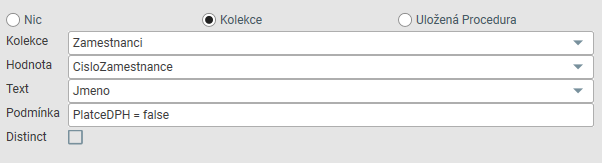
\includegraphics{Figures/cds.png}
				\caption{Tohle je ukázka nastavení CSD 1. typu.}
    			\label{fig:CSDimg}
			\end{figure}
			
			Pro uživatele by CSD z obrázku \ref{fig:CSDimg} vypadal jako combobox jmen zaměstnanců co mají PlatceDPH nastaveno na false, proceduře by se ale poslalo CisloZamnestnance místo jména.
			
			Druhý typ CSD je předem připravená procedura, pro složitější dotazy (např. když je nutno použít join) je potřeba vytvořit proceduru která bude vracet páry textu a hodnot.
		\subsubsection{Akce}
			TODO!!
			
\section{Využité a scházející znalosti a dovednosti}
	\subsection{Využité znalosti}
		\Csharp
		
		asp.net
	\subsection{Scházející znalosti}
		WPF 
		
		async
		
\section{Závěr}
TODO!!


\printbibliography[title={Literatura}, heading=bibintoc]


%\appendix
%\section{}
%TODO!!

\end{document}
